\chapter{Problem definition and background}\label{chapt:problem}
Road digitisation is an expensive operation. Research is being done to identify roads automatically using Artificial Intelligence~(AI) with the different types of images. High-resolution satellite images are expensive to get, and covering an entire state or country is a nightmare. On the other hand, mid-resolution satellite images can be obtained for free, but the identification of roads on mid-resolution~(>~5~m) satellite data is difficult and often has low accuracy. This work tries to detect the smaller roads~(with 1 or 2 lanes), which are often missed.

We will be using RGB images from satellite \href{https://sentinel.esa.int/web/sentinel/missions/sentinel-2}{Sentinel-2A}. \Cref{tab:sentinel-resolution} lists the detailed parameters of the satellite. Band 2 (Blue), 3 (Green), and 4 (Red) are stacked together to get a 3-channel RGB image. As seen in the specifications, the spacial resolution of the final image is 10~m. The task is to increase the accuracy of the existing road-detection algorithm.

\begin{table}[h!]
  \centering
  \begin{tabular}{ |c|c|c| }
    \hline
    Spatial resolution~(m) & Band number & Central wavelength~(nm) \\
    \hline
    10&2&492.4 \\
    10&3&559.8 \\
    10&4&664.6 \\
    10&8&832.8 \\
    20&5&704.1 \\
    20&6&740.5 \\
    20&7&782.8 \\
    20&8a&864.7 \\
    20&11&1613.7 \\
    20&12&2202.4 \\
    60&1&442.7 \\
    60&9&945.1 \\
    60&10&1373.5 \\
    \hline
  \end{tabular}
  \caption[Wavelengths and bandwidths of the three spatial resolutions of the MSI instruments]{Wavelengths and bandwidths of the three spatial resolutions of the MSI instruments~\cite{sentinelSpecifications}.}
  \label{tab:sentinel-resolution}
\end{table}

By combining the three bands from the raw satellite image, the resulting image size is of the order of 400~MB for one mid-sized city. At first, this may not seem significant in comparison with some of the media files. Yet, handling files of this size in DCNN is a severe issue. Processing large files might be possible for massive supercomputers; however a general workstation has Random Access Memory~(RAM) anywhere from 128 to 256~GBs of RAM, while personal computers range from 8~GB to 32~GBs of RAM. Thus, this image must be divided into several parts so that our algorithms work on a readily available device.

Our input image does not have a sufficiently high resolution to identify small roads. To deal with this problem of pixelization, we will be using two types of models. This setup is shown in \cref{fig:model_complete_without_labels}. Unless specifically mentioned, a model means a combined setup using super-resolution and road-detection models. Data from the input layer goes to the super-resolution model, which is consequently passed to the road-detection model. The final output consists of the predicted road network in the image.

\begin{figure}[h!]
  \centering
  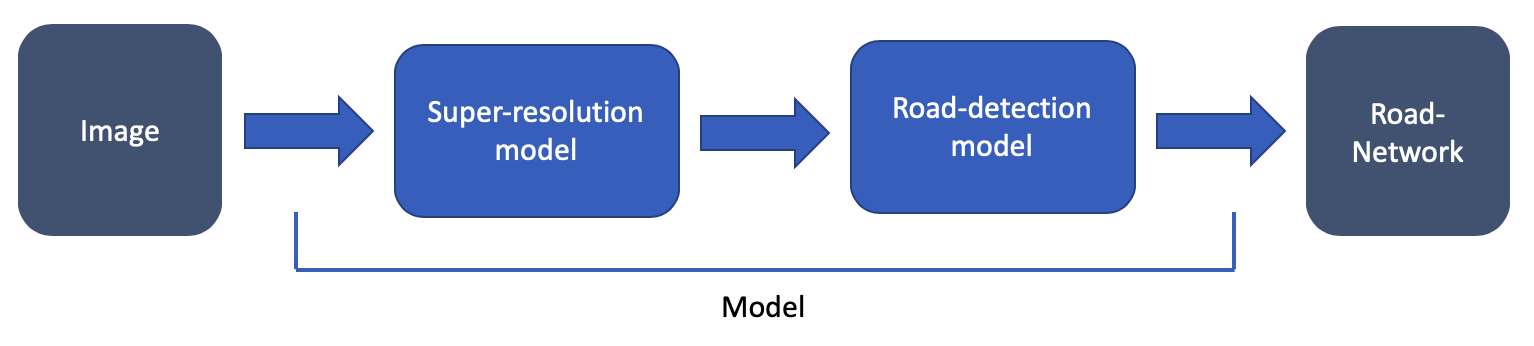
\includegraphics[width=\textwidth]{model_complete_without_labels}
  \caption{Complete setup: Combination of super-resolution and road-detection models.}
  \label{fig:model_complete_without_labels}
\end{figure}
